\begin{figure}[h]
    \centering
    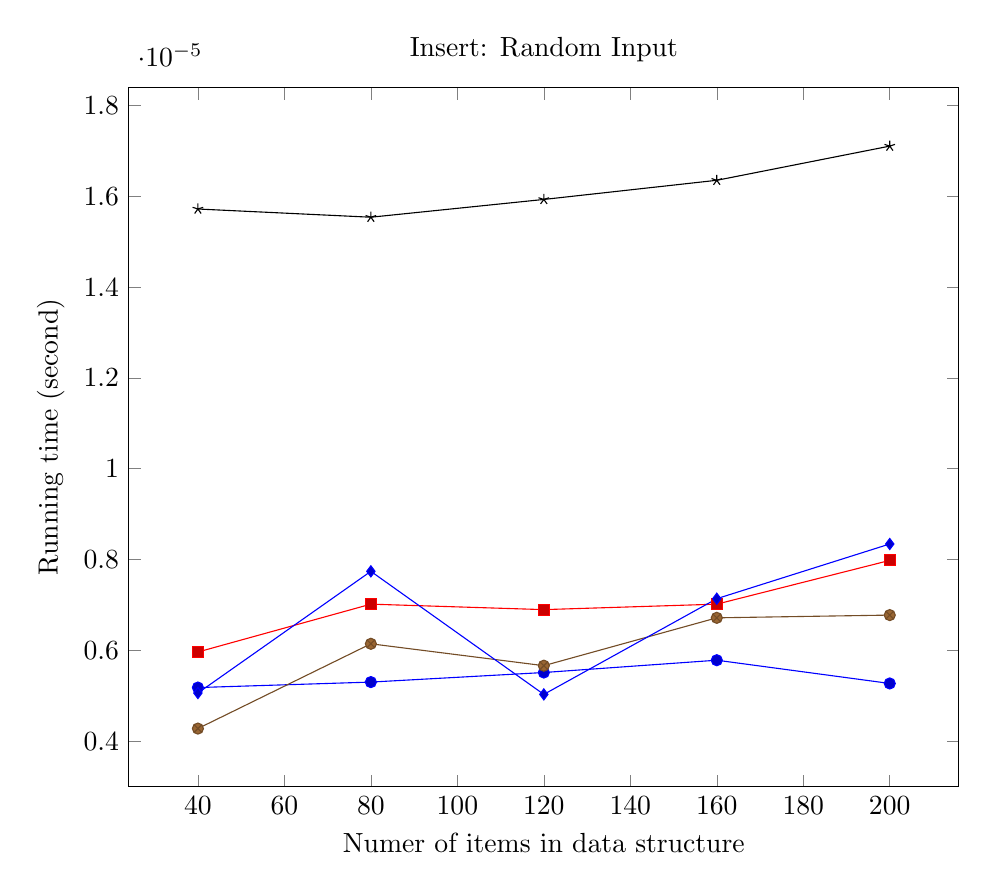
\begin{tikzpicture}
        \begin{axis}[
            xlabel={Numer of items in data structure},
            ylabel={Running time (second)},
            title={Insert: Random Input},
            width=\textwidth
        ]
		\addplot coordinates {
			(40, 5.180215791966703e-06)
			(80, 5.300685926812321e-06)
			(120, 5.511508662436882e-06)
			(160, 5.782566465484251e-06)
			(200, 5.270568393100916e-06)
		};
		\addplot coordinates {
			(40, 5.9632716673974075e-06)
			(80, 7.017385346230754e-06)
			(120, 6.896915211385135e-06)
			(160, 7.017385346230754e-06)
			(200, 7.981146423929886e-06)
		};
		\addplot coordinates {
			(40, 4.2766897820456505e-06)
			(80, 6.1439768700211065e-06)
			(120, 5.662096330993905e-06)
			(160, 6.716210009471979e-06)
			(200, 6.776445077250059e-06)
		};
		\addplot coordinates {
			(40, 1.5721352578523805e-05)
			(80, 1.554064737625538e-05)
			(120, 1.5932175314148367e-05)
			(160, 1.635382078575276e-05)
			(200, 1.710675912747206e-05)
		};
		\addplot coordinates {
			(40, 5.059745657476355e-06)
			(80, 7.74020615459392e-06)
			(120, 5.029628123764951e-06)
			(160, 7.1378554810763715e-06)
			(200, 8.34255682811147e-06)
		};
        \legend{}
        \end{axis}
    \end{tikzpicture}
    \caption{Average of 0 operations, benchmarked every 0, starting at 0.}
\end{figure}